\documentclass[a4paper,12pt]{book}%,twocolumn
%\documentclass[a4paper,11pt]{article}
%% packages

\usepackage{blindtext} % needed for creating dummy text passages
%\usepackage{ngerman} % needed for German default language
\usepackage{amsmath} % needed for command eqref
\usepackage{amssymb} % needed for math fonts
\usepackage[colorlinks=true,breaklinks]{hyperref} % needed for creating hyperlinks in the document, the option colorlinks=true gets rid of the awful boxes, breaklinks breaks lonkg links (list of figures), and ngerman sets everything for german as default hyperlinks language
\usepackage[hyphenbreaks]{breakurl} % ben�tigt f�r das Brechen von URLs in Literaturreferenzen, hyphenbreaks auch bei links, die �ber eine Seite gehen (mit hyphenation).
\usepackage{xcolor}
\definecolor{c1}{rgb}{0,0,1} % blue
\definecolor{c2}{rgb}{0,0.3,0.9} % light blue
\definecolor{c3}{rgb}{0.3,0,0.9} % red blue
\hypersetup{
    linkcolor={c1}, % internal links
    citecolor={c2}, % citations
    urlcolor={c3} % external links/urls
}
%\usepackage{cite} % needed for cite
\usepackage[square,authoryear]{natbib} % needed for cite and abbrvnat bibliography style
\usepackage[nottoc]{tocbibind} % needed for displaying bibliography and other in the table of contents
\usepackage{graphicx} % needed for \includegraphics 
\usepackage{longtable} % needed for long tables over pages
\usepackage{bigstrut} % needed for the command \bigstrut
\usepackage{enumerate} % needed for some options in enumerate
%\usepackage{todonotes} % needed for todos
\usepackage{makeidx} % needed for creating an index
\makeindex
\usepackage{gensymb}
\usepackage{url}
\usepackage{psfrag}
\usepackage{multirow}
\usepackage{subfigure}
%% page settings

\usepackage[top=20mm, bottom=20mm,left=20mm,right=20mm]{geometry} % needed for page border settings
\parindent=0mm % for space of first line of new text block
\sloppy % for writing with hyphenless justification (tries to)
\hyphenation{} % use hyphenation of tolerance parametershttp://www.jr-x.de/publikationen/latex/tipps/zeilenumbruch.html
\hyphenpenalty=10000
\exhyphenpenalty=10000
\usepackage{fancyhdr} % needed for head and foot options
%% my macros

%% Text fomats
\newcommand{\tbi}[1]{\textbf{\textit{#1}}}

%% Math fonts
\newcommand{\bbA}{\mathbb{A}}
\newcommand{\bbB}{\mathbb{B}}
\newcommand{\bbC}{\mathbb{C}}
\newcommand{\bbD}{\mathbb{D}}
\newcommand{\bbE}{\mathbb{E}}
\newcommand{\bbF}{\mathbb{F}}
\newcommand{\bbG}{\mathbb{G}}
\newcommand{\bbH}{\mathbb{H}}
\newcommand{\bbI}{\mathbb{I}}
\newcommand{\bbJ}{\mathbb{J}}
\newcommand{\bbK}{\mathbb{K}}
\newcommand{\bbL}{\mathbb{L}}
\newcommand{\bbM}{\mathbb{M}}
\newcommand{\bbN}{\mathbb{N}}
\newcommand{\bbO}{\mathbb{O}}
\newcommand{\bbP}{\mathbb{P}}
\newcommand{\bbQ}{\mathbb{Q}}
\newcommand{\bbR}{\mathbb{R}}
\newcommand{\bbS}{\mathbb{S}}
\newcommand{\bbT}{\mathbb{T}}
\newcommand{\bbU}{\mathbb{U}}
\newcommand{\bbV}{\mathbb{V}}
\newcommand{\bbW}{\mathbb{W}}
\newcommand{\bbX}{\mathbb{X}}
\newcommand{\bbY}{\mathbb{Y}}
\newcommand{\bbZ}{\mathbb{Z}}
\usepackage{algpseudocode}
\usepackage{float}
\begin{document}

\begin{titlepage}
\center % Center everything on the page

%-------------------------------------------------------------------------------------
%	HEADING SECTIONS
%------------------------------------------------------------------------------------
\textbf{\Large L.E. Robotics (Pvt.) Ltd.}\\[0.5cm]
\textbf{\large No. 100/4, Divulapitiya Road, Minuwangoada,	Sri Lanka}\\[2cm]


\includegraphics[width=0.3\textwidth]{figures/logoler}\\[2cm]

	
%-------------------------------------------------------------------------------------
%	TITLE SECTION
%------------------------------------------------------------------------------------
\textbf{\Huge Machine Vision based\\ Real Time Trajectory Generation\\ (MVbR2TG)}\\[6cm]
%\textbf{\Large A comparison}\\[7cm]


%----------------------------------------------------------------------------------------
%	MEMBERS SECTION
%----------------------------------------------------------------------------------------


\vfill

\begin{tabular}[!h]{ l l}
\textbf{\large Prepared by} & {\large Thalagala B.P.}\\
\textbf{\large Last Modified on}&  {\large \today}
\end{tabular}

%\textbf{\large Prepared by}\\[0.5cm]
%{\large Thalagala B.P.}\\[1cm]
%
%%----------------------------------------------------------------------------------------
%%	DATE SECTION
%%----------------------------------------------------------------------------------------
%\textbf{\large Last Modified on}\\[0.5cm]
%\textbf{\Large \today} % Date, change the \today to a set date if you want to be precise

%----------------------------------------------------------------------------------------


\end{titlepage}
\tableofcontents




\chapter{Feasibility Study}
\section{Introduction}
Most of the robotic arms used in industrial environments operate in a pre-programmed cycle. When it comes to the way a human does the same task is much different as the path planning for picking an object may change from cycle to cycle because of the perception obtained through human vision.\\

Machine vision is the technology and methods incorporated to mimic the human vision in order to gain the insights about the operating environment of the robotics system. However, when it comes to the real time object detection using machine vision, there is an inevitable trade-off between the accuracy and the speed of the operation. This depends entirely on the used machine vision algorithms and the computational power of the available hardware.

\section{Challenges Encountered when Incorporating  a Vision Unit to a Robotic System}

If the robotic system/ arm in interest is not controlled through a dedicated industrial PC with adequate computational resources, the amount of resources that can be allocated to the vision unit becomes limited.  This will eventually result in great delays (which is not desirable when it comes to real time operations) to produce the required outputs by processing the acquired images through the associated camera.\\

Due to this limitation in computational resources it is not practical to use Deep Learning based algorithms in time critical industrial applications. Because, by the time the decisions are made the environment may have already changed and the made decisions may no longer valid.
\pagebreak
\section{A Traditional Machine Vision Approach as the Solution}

To overcome the challenges mentioned above traditional machine vision algorithms can be incorporated inside the vision unit. Unlike the deep learning based algorithms, traditional machine vision algorithms  are less computationally expensive and no initial data is require to train the algorithm. As they are build upon strong mathematical foundation they work well in almost all the situations when the parameters are tuned properly.

\section{High Level Representation of the Algorithm}

For real time trajectory generation we first need to track the objects on the conveyor belt. A typical object tracking framework generally consists of three major modules which can be identified as, 1. Object Detection, 2. Object Modeling and 3. Object Tracking. The following traditional computer vision methods will be used to implement those three modules.\\

\begin{table}[!h]
	\centering
	\begin{tabular}[!h]{|l | l|}
		\hline
		\textbf{Module} & \textbf{Method}\\
		\hline
		Object Detection &  Connected Component Analysis and Background Subtraction\\
		Object Modeling & Contour Analysis and Representation\\
		Object Tracking & Template Matching followed by Object moments interpretation\\ 
		\hline\hline
	\end{tabular}
\caption{Modules of a Typical Object Tracking Framework}
\end{table}
	
%Pseudo code representation of the functioning of above three modules cane be expressed as follows.
%
%
%\begin{verbatim}
%1. Capture an image of a sample object placed on the conveyor belt
%2. Create the `template image' using that image
%3. While True
%4. 	Capture a frame
%5. 	Convert the frame to a grayscale image
%6. 	Thresholding the image for segmentation
%7. 	Connected compponent Analysis
%8. 	Background Subtraction
%9. 	Contour Analysis to identify the object Contorurs
%10. Template matching 
%\end{verbatim}

Through the above framework we can identify and track the centroids of the objects on the conveyor belt and that information cam be handed over to the trajectory generation algorithm to generate the required path in the real time  to pick the object. Following subsections highlights the contribution from the each module tabled above where a conveyor belt which carries hexagonal nuts is used as the example.

\begin{figure}[H]
	\centering
	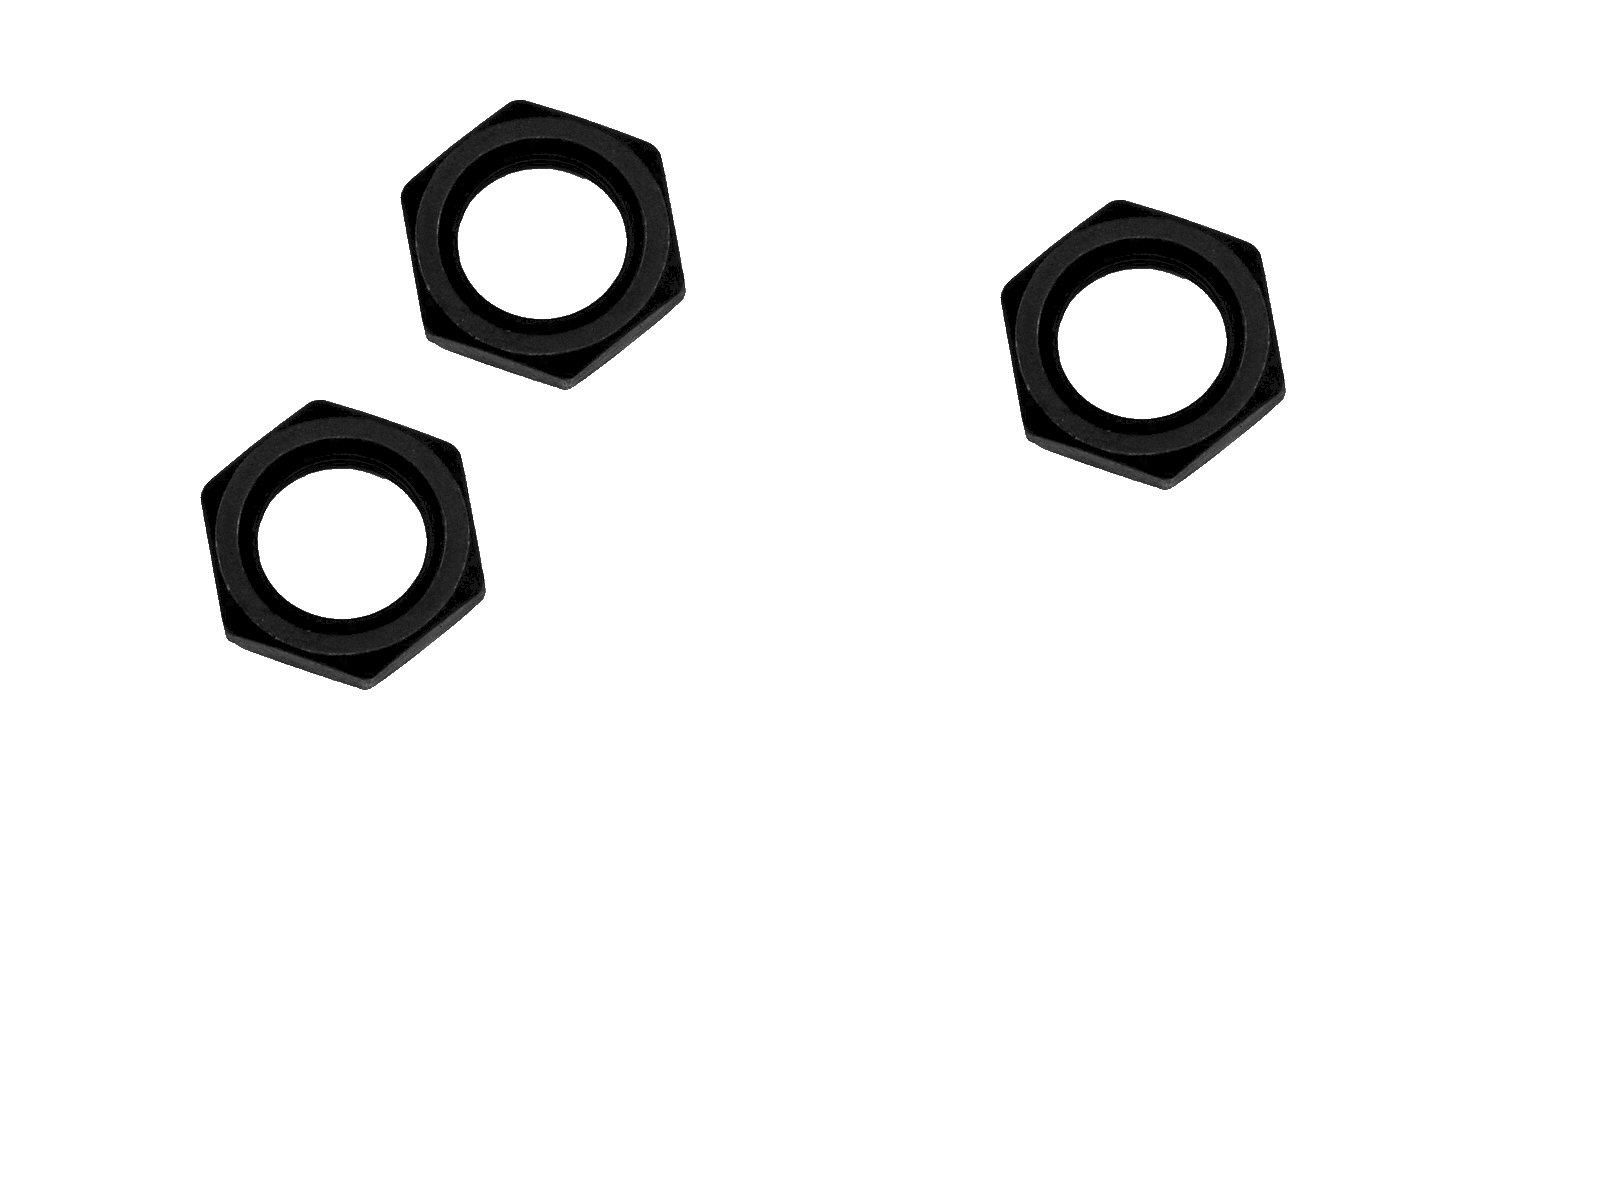
\includegraphics[scale=0.17]{figures/belt}
	\caption{Single frame of the video captured from the camera}
\end{figure}


\subsection{Object Detection: Connected Component Analysis (CCA) and Background Subtraction}

As the first step of the object detection and tracking, the foreground (objects) must be separated from the background. This segmentation is done at this stage  using \textit{connected component analysis} (CCA). Through the CCA different connected objects found in the image can be assigned different labels. Those label information can then be used to subtract the background from the  image. Prior to CCA, thresholding followed by a suitable morphological transformation must be done. For this example \textit{Otsu's thresholding} and \textit{morphological closing} are used.

\begin{figure}[H]
	\centering
	\subfigure[Labeling of connected objects using CCA]
	{ 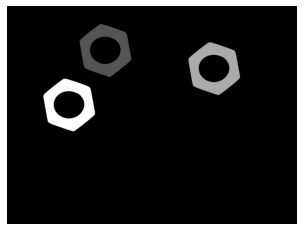
\includegraphics[scale=0.65]{figures/cca}
	}\hspace{5mm}
	\subfigure[Subtracting the background]
	{ 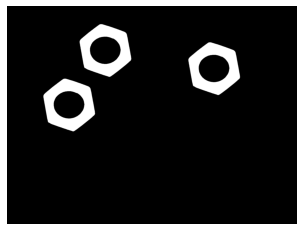
\includegraphics[scale=0.65]{figures/backsub}
	}
\caption{Connected Component Analysis (CCA) and Background Subtraction}
\end{figure}

\subsection{Object Modeling: Contour Analysis and Representation}

Background subtracted image is used in this stage to find contours. These contours can be then used as a representation of the objects on the conveyor belt.

\begin{figure}[H]
	\centering
	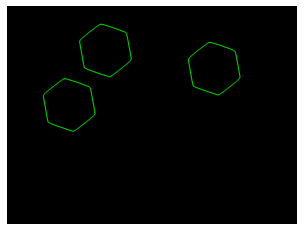
\includegraphics[scale=0.65]{figures/contours}
	\caption{Finding contours in the image}
\end{figure}

\subsection{Object Tracking: Template Matching followed by Object moments interpretation}

In order to identify different objects a procedure called as \textit{template matching} is carried out. For this template matching, reference images known as template images should be created using a properly captured images of the objects that are intended to convey using the conveyor belt. Contours of these templates can be compared with the object contours found in the previous stage to identify similar objects for further processing. 

\begin{figure}[H]
	\centering
	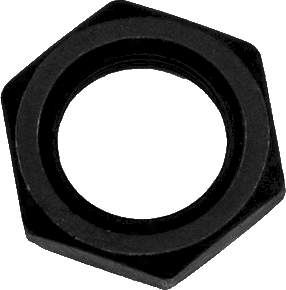
\includegraphics[scale=0.45]{figures/template}
	\caption{Sample template image for a conveyor belt carrying hexagonal nuts}
\end{figure}

%\bibliographystyle{plain}
%\bibliography{refer}

%---------------------------------------------------------------------------
\end{document}
